\documentclass[letterpaper]{article}
\usepackage{natbib,alifexi}
\usepackage[inline]{enumitem}
\usepackage[utf8]{inputenc}
\usepackage[T1]{fontenc}
\usepackage{url}
\usepackage{amsmath}
\usepackage{amsfonts}
\usepackage{amsthm}
\usepackage{cases}
\usepackage[inline]{enumitem}
\newcommand*{\codeinl}{\texttt}

\theoremstyle{definition}
\newtheorem*{definition}{Definition}
\newtheorem*{notation}{Notation}
\theoremstyle{remark}
\newtheorem*{note}{Note}
\newtheorem*{example}{Example}

\title{Pitch Shifting of Music Signals}
\author{Théo Verhelst \\ Université Libre de Bruxelles}

\begin{document}
\maketitle

\begin{abstract}
Pitch shifting is the task of modifying the frequency of a signal while keeping
its duration intact. Pitch shifting is an important feature of many digital
music tools, and needs to be done in real-time with the highest available
quality. In this report, we describe state-of-the-art techniques of pitch
shifting, and we explain in detail one that is particularly suited to music
signals. This technique uses phase vocoder for time-scaling and 3rd order spline
interpolation for resampling. We also describe a Clojure implementation of this
technique.
\end{abstract}

\section{Introduction}
\emph{Pitch shifting} is a process that changes the frequency of a signal
without modifying its duration. The main difficulty of pitch shifting is to make
the synthesised signal as natural as the original, so that it sounds like as if
it was recorded or created on this new pitch. More precisely, the timbre and the
duration of the signal need to be preserved.

\paragraph{}
One application of pitch shifting is to change the pitch of an instrument
recording in a music production software, in order to tune it to the other
instruments, or for any other musical purpose. Another widespread use of pitch
shifting is in DJ software \citep{Cliff00hangthe}: one can change the pitch of a
track, and therefore its key, in order to make the transition to the next track
easier and smoother.

\paragraph{}
The most straightforward way to change the pitch of an audio signal is to
resample the signal at another sampling rate, and playing it back at its
original rate. But both pitch and duration are modified at the same time. Thus,
we need a more sophisticated technique in order to preserve the duration
constant \citep{DM}.

\paragraph{}
In contrast to pitch shifting, \emph{time-scale modification} (\emph{TSM}) is a
process that modifies the duration of a signal without modifying its pitch and
its timbre. TSM has been subject to many more studies than pitch shifting.
However, we base our work on these studies, since it is possible to show that
both processes are mathematically equivalent. Indeed, in order to change the
pitch of a signal, one can use a well-known TSM method, and then resample the
signal.

\section{Time-scale modification techniques}
TSM techniques can be grouped in two main categories: \emph{time-domain TSM} and
\emph{frequency-domain TSM}.

\paragraph{}
Time-domain TSM extracts portions of the input signal at a frequency defined by
the scaling factor, and places them in the output signal. This technique is
particularly suited to monophonic, harmonic signal, as it preserves almost
perfectly the timbre of the signal. The basic time-domain algorithm,
\emph{overlap-and-add} (or \emph{OLA}), suffers from phase jumps artifacts, but
there are many variations of this algorithm that avoid this effect. But all of
them are only able to correct phase jumps on the most prominent frequency, i.e.
the fundamental frequency of the signal. Phase jumps can still occur in less
important frequencies, i.e. the harmonics, which is clearly audible. OLA-base
algorithms are thus not suited to polyphonic signals, since they contains more
harmonics than monophonic ones. Furthermore, non-harmonic signals, such as drums
or percussive instruments, have non-periodic patterns. These patterns are known
as \emph{transients}. A typical time-domain TSM technique leads to transient
doubling or skipping (depending on the scaling factor), since these techniques
periodically repeat or discard some small parts of the signal. This can be
reduced by taking a very short frame size, or managing separately the transients
after a transient detection procedure \citep{Grofit2008}.

\paragraph{} Frequency-domain TSM is based on the short-time Fourier transform
(STFT). It splits the signal in small chunks, and computes the Fourier transform
of each of these chunks, in order to get a discrete frequency-domain
representation of the signal. Often, the technique also uses the \emph{phase
vocoder} in order to refine the frequencies estimates, and are thus named
\emph{phase-vocoder time-scale modification}, or \emph{PV-TSM}, or simply phase
vocoder. The idea is to preserve phase continuity across all frequencies, and
not only on the most prominent frequency as in time-domain TSM, by exploiting
the frequency-domain representation of the sound. PV-TSM behaves well on
polyphonic signals, but are subject to vertical phase incoherence, i.e. the
relationship between the phases of different frequencies at a point of time is
not preserved, leading to audible artifacts, known as \emph{phasiness}, or
\emph{loss of presence}.

\section{General procedure}
\label{sec:procedure}
Pitch shifting process is split in two steps: \begin{enumerate*}[label=\arabic*)]
\item apply a TSM procedure \item resample the signal\end{enumerate*}. Let
\(\alpha\) be the scaling factor. We first apply a TSM procedure with parameter
\(\alpha\), so that the playback speed is modified, while the pitch is left
unmodified. Then, we resample the signal by a factor \(1/\alpha\), so that the
playback speed of the signal is the same as the original, but the pitch is
multiplied by \(\alpha\).

\paragraph{}
For the TSM part, we use a simple phase vocoder with phase propagation. For the
resampling part, we use an interpolator based on 3rd order splines. These are
explained below.

\section{Time-scale modification}
\subsection{Basics of time-scale modification}
\begin{notation}
	Let
	\[[a:b]:=\{a,a+1,\dots,b-1,b\}\quad\forall a,b\in\mathbb{Z}:a<b\]
	and
	\[[a:b[\;:=\{a,a+1,\dots,b-1\}\quad\forall a,b\in\mathbb{Z}:a<b\]
\end{notation}

\paragraph{}
First, we have to define the basic concepts involved in time-scaling. Let the
function \(x:\mathbb{Z}\to[-1, 1]\) be signal to time-scale. In practice,
the analysed audio signal has a finite duration of \(L\in\mathbb{N}\) samples.
Thus we define \(x(n)=0\,\forall n\in\mathbb{Z}\setminus [0:L[ \) for the sake
of simplicity. We want to construct the output signal
\(y:\mathbb{Z}\to[-1, 1]\) that have the same frequency-domain properties as
\(x\), but being stretched in time by the factor \(\alpha\).

\paragraph{}
Almost all TSM techniques are based on the following procedure: first, \(x\)
is divided in \emph{analysis frames} \(x_m,\,m\in\mathbb{Z}\) having each a
length of \(N\) samples, and these analysis frames are spaced by an
\emph{analysis hop size} \(H_a\):
\begin{equation}x_m(n)=\begin{cases}
	x(mH_a + n) & \text{if }n\in [0:N[ \\
	0           & \text{otherwise}
\end{cases}\end{equation}
Then, we could want to put these frames in the output signal by spacing them
with another hop size, which we name \emph{synthesis hop size} \(H_s\), thus
changing the overall duration of the signal. But this would cause very audible
phase discontinuities, since the end of a frame would no longer match with the
beginning of the next frame. Thus, we need to modify the analysis frames \(x_m\)
into \emph{synthesis frames} \(y_m\) before adding them to the output signal
\(y(n)\):
\begin{equation}
	y(n) = \sum_{m\in\mathbb{Z}}y_m(n-mH_s)
\end{equation}
\begin{figure}[h]
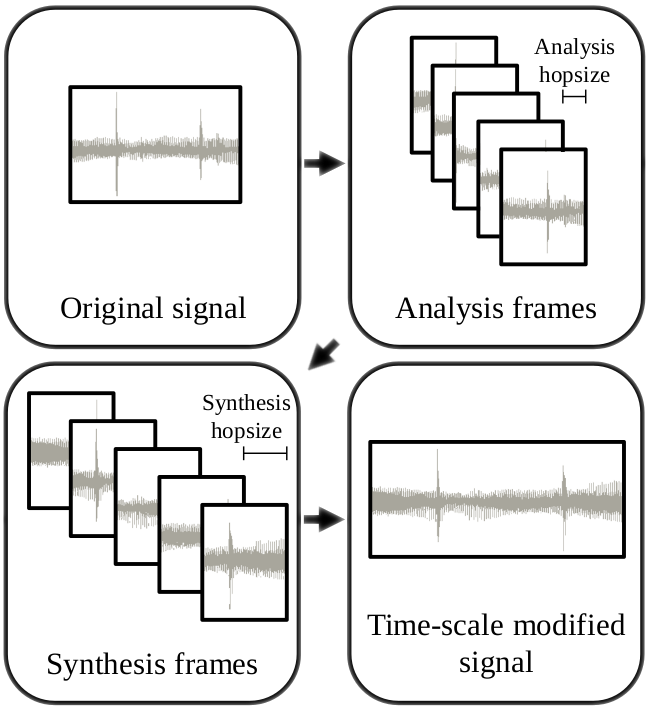
\includegraphics[width=\linewidth]{pipeline.png}
\caption{General procedure of time-scale modification.}
\end{figure}

\paragraph{}
\(H_s\) is usually set to \(N/2\) or \(N/4\), in order to have a constant
overlap between the synthesis frames. And since we know that
\(\alpha=\frac{H_s}{H_a}\), we then have \(H_a=\frac{H_s}{\alpha}\).

\paragraph{}
The method used to transform \(x_m\) into \(y_m\) is critical, as it determines
the quality of the result. In addition to phase discontinuities, it must also
compensate gain fluctuations: if no care is taken, two overlapping frames may
have a higher gain in the overlapping part than in the rest of the signal.
A common procedure to compensate gain fluctuations is to multiply each modified
frame by a windowing function \(w:\mathbb{N}\to[0,1]\) before adding them to the
output signal \(y\):
\begin{equation}
	\label{synthesis}
	y(n) = \sum_{m\in\mathbb{Z}}
	\frac{w(n-mH_s)y_m(n-mH_s)}
	{\sum_{k\in\mathbb{N}}w(n-(m + k)H_s)}
\end{equation}
The numerator of the fraction is simply the product of the synthesis frame with
the window function, while the denominator scales the gain amplification that
may be induced by the use of the window function. The Hann window is a common
choice as a window function, and is defined as
\begin{equation}
\label{hann}
w(n)=\begin{cases}
	0.5(1-cos(\frac{2\pi n}{N-1}))\text{ if }n\in[0:N[\\
	0 \text{ otherwise}\end{cases}
\end{equation}
The Hann window has the property that if we add Hann windows spaced by \(N/2\)
in their domain, the sum of the overlapping parts we be equal to one:
\begin{equation}
	\forall n\in\mathbb{Z}\quad\sum_{i\in\mathbb{Z}}w(n + i\frac{N}{2}) = 1
\end{equation}
This property allows to add windowed signal frames without gain multiplication,
given that the synthesis hopsize is half the frame length. Note that in this
case, the denominator of \eqref{synthesis} reduces to \(1\).
\begin{figure}[h]
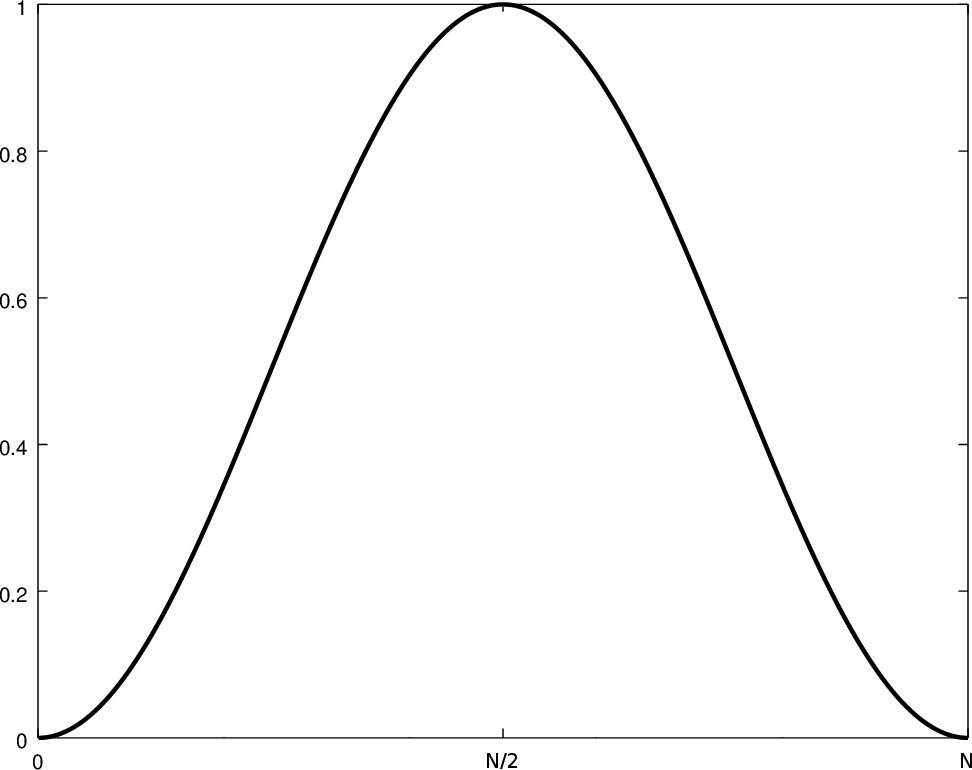
\includegraphics[width=\linewidth]{hann.png}
\caption{The Hann window function.}
\end{figure}

\subsection{Phase-vocoder time-scale modification}
The phase vocoder is a common frequency-domain technique used to derive the
\emph{synthesis frames} \(y_m\)  from the analysis frames \(x_m\). The idea is
to compute the spectrum of the frame with the Fourier transform, and change the
phases of this spectrum so that the signal re-synthesised from this modified
spectrum has no phase jump with the following and previous frames.

\paragraph{Short-time Fourier transform}
The spectrum of a signal is the frequency-domain representation of a time-domain
signal, and is composed by the amplitudes and phases of the Fourier series
decomposition of the signal. The Fourier transform of discrete-time signals is
primarily defined for signals of length \(N\) \citep{bracewell1986fourier}:
\begin{equation}
	X(k) = \sum_{n=0}^{N-1}x(n)\exp(-2\pi ikn/N)
\end{equation}
where \(k\in [0:N[\) denotes the frequency index (see \eqref{frequency_index}).
This yields \(N\) complex numbers, where \(|X(k)|\) is the magnitude of the
\(k\)th frequency, and \(\arg(X(k))\in[0,1[\) is the phase of the \(k\)th
frequency. Note that we use phases in the unit range because we also manipulate
frequencies in Hertz, and we don't want to divide the phase by \(2\pi\) each
time we use it in an equation involving a frequency. Thus, we have
\begin{equation}
	X(k)= |X(k)|\exp(2\pi \text{i} \arg(X(k)))
\end{equation}

\paragraph{}
As required by the time-scaling algorithm, we will apply the Fourier transform
on small portions of the signal. We could want to do apply directly the
transform on analysis frames \(x_m\):
\begin{equation*}
X(m,k)=\sum_{n=0}^{N-1}x_m(n)\exp(-2\pi ikn/N)
\end{equation*}
But this can lead to unexpected high amplitudes in the high frequencies: the
Fourier transform works as if the signal was periodic with a period \(N\)
\citep{Dolson1986}, i.e. as if we where computing the Fourier series of a signal
\begin{equation}
\tilde x:\mathbb{Z}\to\mathbb{R}:n\mapsto x_m(n\mod N)
\end{equation}
which can have high amplitude in high frequencies around
\(n=aN\;\forall a\in\mathbb{Z}\).
A solution is to apply a windowing function to the analysis frame, so that the
signal is always zero at the frame boundaries \citep{gabor1946theory}:
\begin{equation}
	X(m,k) = \sum_{n=0}^{N-1}x_m(n)w(n)\exp(-2\pi ikn/N)
\end{equation}
\(X(m,k)\) is the coefficient of the \emph{short-time Fourier transform} of
the signal \(x\) at time \(m\) and at frequency \(k\). It is also named a
\emph{time-frequency bin}. \(w\) is a windowing function, usually the Hann
window as defined in \eqref{hann}

\paragraph{}
Note that the frequency index \(k\) corresponds to the physical frequency
\begin{equation}
	\label{frequency_index}
	F_{\text{coef}}(k) = \frac{F_s k}{N}
\end{equation}
where \(F_s\) is the sampling rate in Hz, and the frame index \(m\) corresponds
to the physical time
\begin{equation}
	T_{\text{coef}}(m) = \frac{H_a m}{F_s}
\end{equation}

\paragraph{Synthesis with modified frames}
Our goal is to compute the synthesis time-frequency bins \(Y(m,k)\) from the
analysis time-frequency bins \(X(m,k)\), so that the signal synthesised with the
inverse Fourier transform from these synthesis time-frequency bins has phase
coherence from one frame to the next. Since we are only interested in phase
adjustment, we can already set
\begin{equation}
	|Y(m,k)| = |X(m,k)|
\end{equation}
We also have to determine the phase \(\arg(Y(m,k))\), so that we can synthesise
the synthesis frame \(y_m\) from the synthesis time-frequency bins \(Y(m,k)\).
Note that the modified STFT may not be invertible, i.e. there may be no signal
\(y\) whose STFT is \(Y(m,k)\). However, there is a procedure described in
\citep{signalEstim} that minimizes the squared error between \(Y(m,k)\) and the
STFT of the resulting signal. It results that the synthesis frame \(y_m\) is
given by:
\begin{equation}
	\label{modified_synth}
	y_m(n)=\frac{1}{N}\sum_{k=0}^{N-1}Y(m,k)\exp(2\pi\text{i}kn/N)
\end{equation}
We can then reconstruct the output signal \(y\) with the equation
\eqref{synthesis}.

\begin{figure}[h]
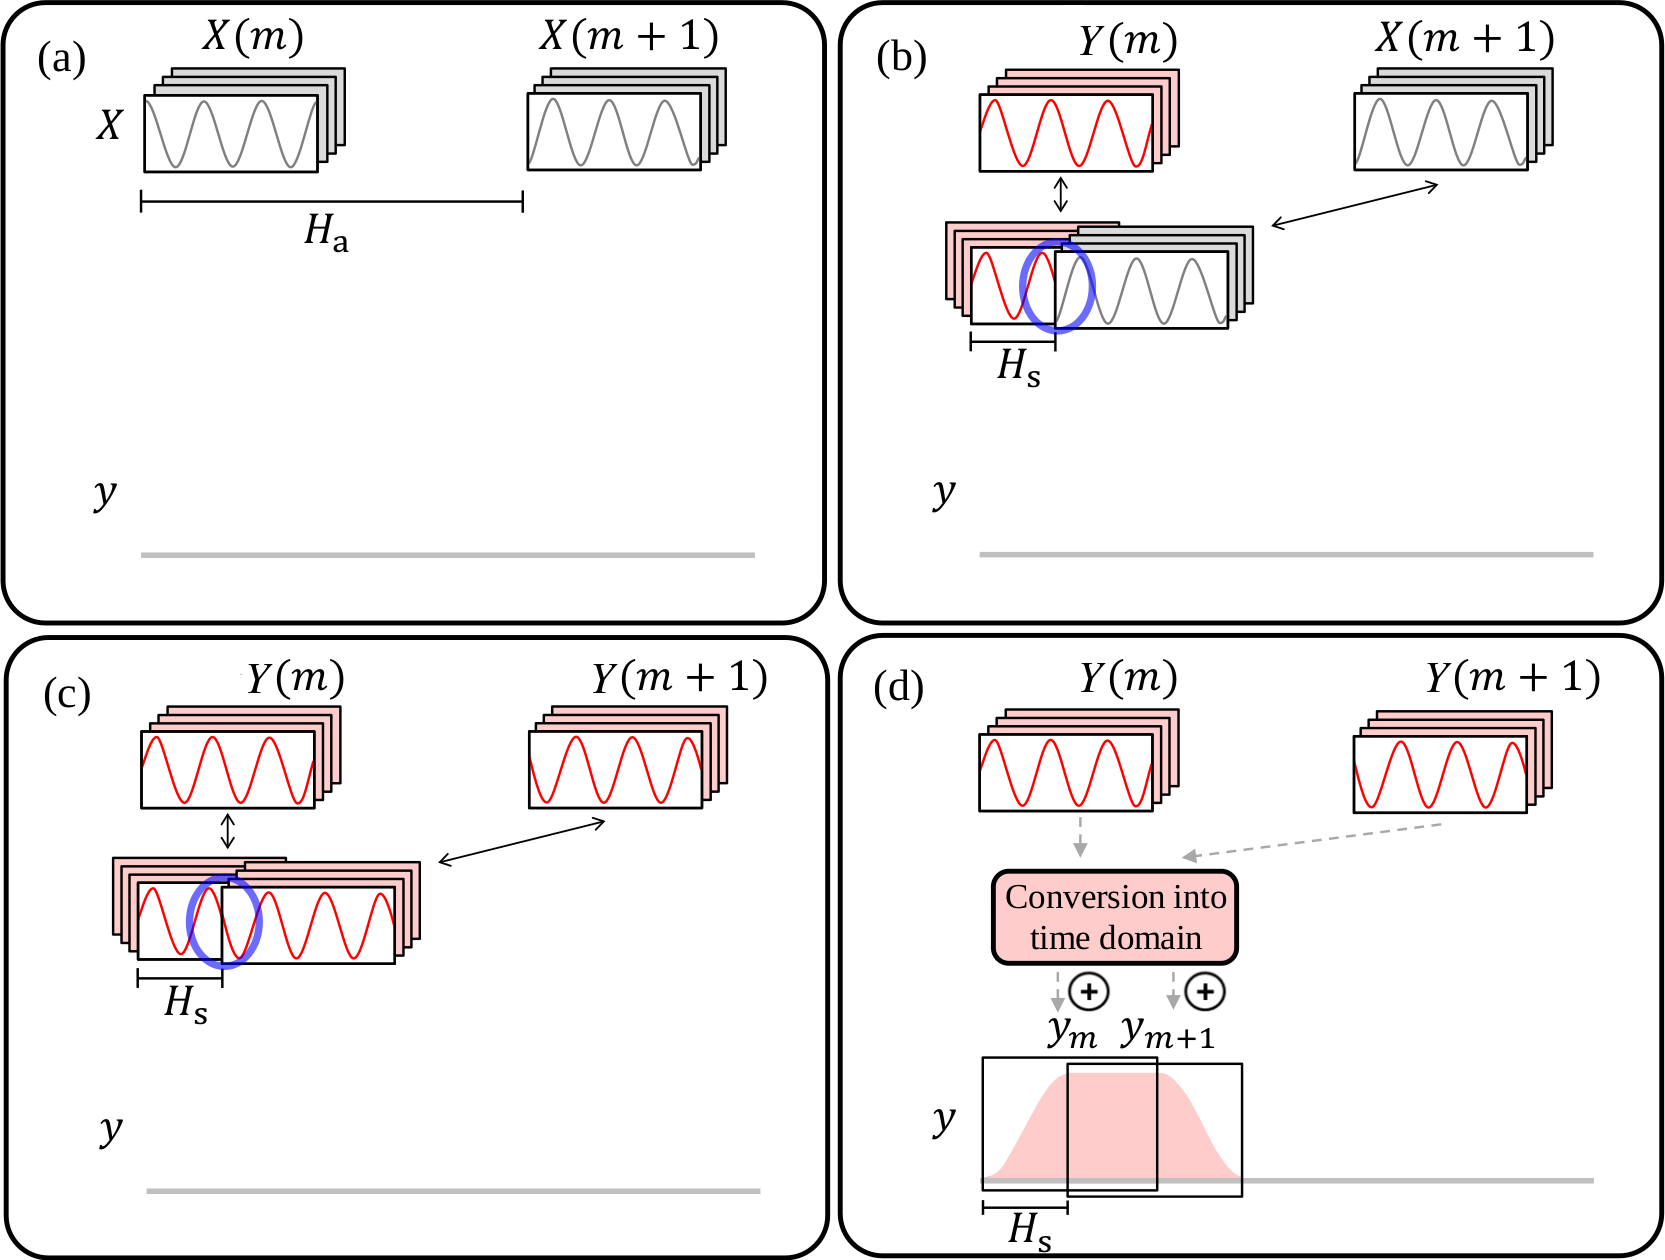
\includegraphics[width=\linewidth]{phase-vocoder.png}
\caption{The phase-vocoder procedure.
	\begin{enumerate*}[label={(\alph*)}]
	\item The input signal is analysed and its STFT is calculated;
	\item The previous modified time-frequency bin is compared with the current
	unmodified time-frequency bin;
	\item The phase of the previous time-frequency bin is used to adjust the phase
	of the current one;
	\item The modified time-frequency bins are converted back into time-domain and
	overlapped.
	\end{enumerate*}
}
\end{figure}

\paragraph{Instantaneous frequency}
The phase adjustment involves the observation that the short-time Fourier
transform yields coefficients for a finite quantity of frequencies, and that may
be insufficient to characterise exactly the underlying sinusoids involved in the
Fourier series decomposition of the signal. However, it is possible to refine
the frequency of the \(k\)th frequency index by using the phases of the current
and next frame. This refined frequency is called the \emph{instantaneous
frequency} and is denoted by \(F_{\text{coeff}}^{\text{IF}}(m,k)\).
\begin{notation}
Let \[\phi_m:=\arg(X(m,k))\]
and \[\gamma_m:=\arg(Y(m,k))\]
\end{notation}
In order to find the instantaneous frequency, we first can observe that for any
time-frequency bin \(X(m,k)\), we can compute its \emph{unwrapped phase
advance}, that is, the phase increment that should occur from the time
\(T_{\text{coef}}(m)\) to the time \(T_{\text{coef}}(m+1)\), according to the
frequency estimate \(F_{\text{coef}}(k)\):
\begin{equation}
	\phi^{\text{inc}}=F_{\text{coef}}(k) \Delta t_a
\end{equation}
where \(\Delta t_a\) is analysis hop time given is seconds:
\begin{equation}
	\Delta t_a=H_a/F_s
\end{equation}
Since we know the phase \(\phi_m\), we can compute the predicted phase at
the time \(T_{\text{coef}}(m+1)\):
\begin{equation}
	\phi^{\text{pred}}_{m+1}=\phi_m + \phi^{\text{inc}}
\end{equation}
But because of the lack of precision of the phase vocoder, this predicted phase
may not be equal to \(\phi_{m+1}\) when mapped in the range \([0, 1[\).
We can then compute the difference with the effective phase \(\phi_{m+1}\), and
this difference is called the \emph{phase error} (or \emph{heterodyned phase
increment}):
\begin{equation}
	\phi^{\text{err}}_m=\Psi(\phi_{m+1} - \phi^{\text{pred}}_{m+1})
\end{equation}
where the function \(\Psi\) is the \emph{principal argument function} that maps
the phase difference to the range \([-0.5, 0.5]\).
Here is a possible implementation of \(\Psi\):
\begin{equation}
	\Psi:\mathbb{R}\to[-0.5,0.5]:\phi\mapsto \phi - \lceil \phi-0.5 \rceil
\end{equation}
From this phase error, we can compute the \emph{instantaneous frequency}: this
is a refinement of \(F_{\text{coef}}(k)\), in an attempt to determine the
frequency of the underlying sinusoid by taking the phase error into account.
This sinusoid should have a phase of
\(\phi_m\) at the time \(T_{\text{coef}}(m)\) and a phase \(\phi_{m+1}\) at
the time \(T_{\text{coef}}(m+1)\).
\begin{align}
	&F_{\text{coeff}}^{\text{IF}}(m,k)=\frac{\phi^{\text{inc}} + \phi^{\text{err}}_m}{\Delta t_a}\\
	&=F_{\text{coef}}(k) + \frac{\phi^{\text{err}}_m}{\Delta t_a}\\
	&=F_{\text{coef}}(k) + \frac{\Psi(\phi_{m+1} - \phi_m - \phi^{\text{inc}})}{\Delta t_a}
\end{align}

\paragraph{Phase adjustment}
Now that we have refined the coarse frequency estimates of the STFT, we can use
this information to adjust the phase of the time-frequency bins. The idea is to
set the phase of the bin according to the phase and the instantaneous frequency
of corresponding bin in the previous frame:
\begin{equation}
	\gamma_m=\gamma_{m-1} + F_{\text{coeff}}^{\text{IF}}(m-1,k)\Delta t_s
\end{equation}
We now use the synthesis hop time since we are synthesising the output frames,
and they are spaced by the synthesis hoptime \(\Delta t_s=H_s/F_s\).

\paragraph{}
This formula recursively defines the modified frame from the previous modified
frame and a refined frequency estimate of the underlying sinusoid. Thus, we
need an initial step for the first frame. In practice, we do not change the
phases of the first frame, since there is no phase discontinuity with the
previous frame:
\begin{equation}
	\label{initial_phase}
	\gamma_0=\phi_0
\end{equation}
Now that we defined all synthesis time-frequency bins, we can use the equation
\eqref{modified_synth} to construct the synthesis frames, and then equation
\eqref{synthesis} to synthesise the final output signal.

\begin{figure}
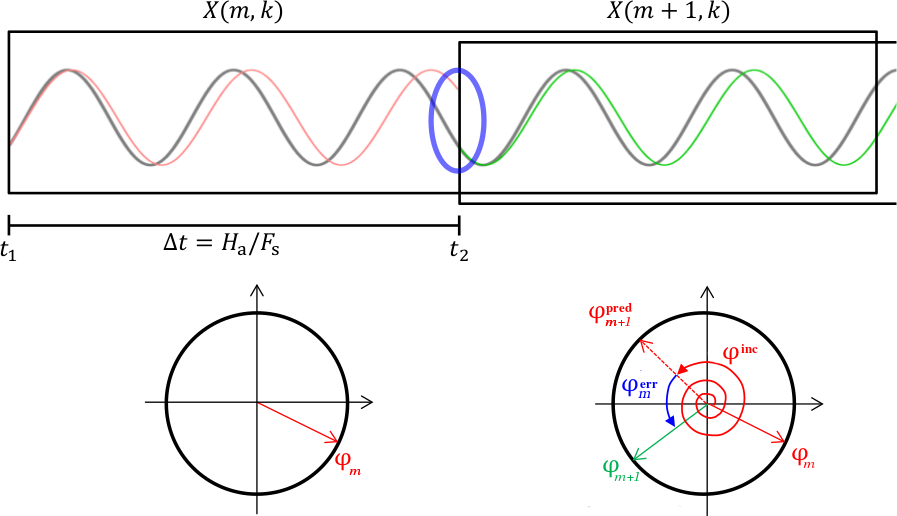
\includegraphics[width=\linewidth]{phase-unwrapping.png}
\caption{The phase adjustement procedure. The difference between the predicted
phase at \(t_2\) (\(\phi^{\text{pred}}_{m+1}\)) and the effective phase given by
the STFT (\(\phi_{m+1}\)) is used to refine the coarse frequency estimate (in
red) to the instantaneous frequency (in grey).}
\end{figure}

\subsection{Result and limitations}
Thanks to the phase modification procedure, the phase continuity is guaranteed
in successive frames, and allows efficient time-scaling of a polyphonic musical
signal. This phase phase continuity in time is called horizontal phase
coherence. But the phase relationship between the frequency channels in one
frame is no longer respected. This relationship is called vertical phase
coherence. This leads to phasiness, and the resulting sound is characteristic of
phase-vocoder techniques \citep{Laroche1999}. Another effect is transient
smearing: in musical signals with percussions, such as drums, the percussive
aspect of the sound results of the subtle and sudden tuning of the phases of
various sinusoids in the signal. And because of the lack of vertical phase
coherence, the percussive aspect of transients is significantly reduced.

\paragraph{}

\subsection{Further improvements}
Many improvements has been proposed to the standard phase-vocoder procedure,
mainly to reduce the phasiness and transient smearing of the result. One of
them \citep{Dorran_audiotime_scale, Kraft2012ImprovedPT}, is based on the
observation that the phasiness increases over time from the time where the
modified phase is set as the initial input phase (see \eqref{initial_phase}).
Thus, by placing periodically in the output signal an analysis frame unchanged,
the vertical phase coherence is reset before it degenerates too much. The
unmodified frame is placed in the signal with usual time-domain procedure,
such as \emph{Waveform Similarity Overlapp and Add} (\emph{WSOLA})
\citep{Verhelst1993}.

\paragraph{}
Another well-known improvement of the standard phase-vocoder has been proposed
by J. Laroche and M. Dolson \citep{Laroche1999}. It is based on the observation
that the phase of a sinusoid is mainly tied to the phase of the nearest peak
in the spectrum. Although phase inconstency between a very low-frequency
sinusoid and a high-pitched one is barely noticeable, a high-amplitude sinusoid
influences the phase of nearby frequency channels. Garbaging this latter
relation results in audible phasiness. The idea of this improved phase-vocoder
is to lock the phase of all frequency channels to the one of the neared peak
in the spectrum. As a result, the vertical phase incoherence is greatly reduced.
Furthemore, the computational cost of the phase-vocoder is also reduced since
the phase propagation has to be computed only for the peak frequencies.

\paragraph{}
J. Driedger and M. Müller presented an hybrid approach to time-scale
modification of music signals, taking advantages of both time-domain and
frequency-domain advantages \citep{DM}. We first separate the signal in
percussive and harmonic content, and then we apply a time-domain procedure with
a short frame length on the percussive component, and a frequency-domain
procedure on the harmonic component, and finally we add both results.
Percussive-harmonic separation can be achieved by applying a median filter
on the time-frequency bins. This procedure benefits from all the improvements
that have been made on the phase-vocoder, while it easily copes with transient
smearing by using an effective time-domain algorithm.

\section{Resampling}
The goal of resampling is to reconstruct a continuous-time signal from the given
discrete-time samples, and then sample this signal again with another sampling
rate. More formally, we want to construct the continuous-time signal
\begin{equation}\hat x:\mathbb{R}\to\mathbb{R}\end{equation}
such that
\begin{equation}x(n) = \hat x(Tn) \;\forall n\in\mathbb{Z}\end{equation}
where \(T\) is the sampling period (the inverse of the sampling rate). Then, we
sample a new signal \(y\) at a sampling period \(T'\):
\begin{equation*}y(n) = \hat x(T'n) \;\forall n\in\mathbb{Z}\end{equation*}

\subsection{Procedure}
In order to construct the continuous-time signal, we need an interpolator. There
exists various interpolators, such as truncated sinc
\citep{duncan1988fundamentals, rossum1989an}, linear-interpolator
\citep{rossum1993}, b-spline interpolator \citep{Sankar1998},
Lagrange interpolator \citep{Schafer1973}. We chose 3rd order Hermite spline
interpolator, for its simple implementation \citep{Grisoni97anhermitian}.

\paragraph{}
For 3rd order spline interpolation, we search the factors of a 3rd-degree
polynomial for each pair of consecutive signal values \((x(n),\,x(n+1))\), such
that this polynomial passes through these values.
\begin{notation}
	Let
	\begin{equation*}
	y_0=x(n-1);\;y_1=x(n);\;y_2=x(n+1);\;y_3=x(n+2)
	\end{equation*}
\end{notation}
We search the interpolating function
\begin{equation}
\label{interpolation_poly}
f:[0, 1]\to\mathbb{R}:t\mapsto \sum_{i=0}^{3}\alpha_i t^i
=\alpha_0+\alpha_1 t+\alpha_2t^2+\alpha_3t^3
\end{equation}
In order to determine the value of the factors \(\alpha_i\), we need to set four
constraints on the function \(f\):
\begin{numcases}{ }
f(0)=y_1\label{constr1}\\
f(1)=y_2\label{constr2}\\
f'(0)=\frac{y_2-y_0}{2}\label{constr3} \\
f'(1)=\frac{y_3-y_1}{2}\label{constr4}
\end{numcases}
\eqref{constr1} and \eqref{constr2} are natural constraints of spline
interpolator: we want that the interpolating function passes through the
supplied values \((x(n),\,x(n+1))\). But in order to determine the factors
\(\alpha_i\), we need two more constraints. One solution is to use Hermite
splines \citep{de1978practical}, that is, the derivative of \(f\) at \(t\in\{0,
1\}\) is equal to the derivative of a straight line between the previous and the
next point (\eqref{constr3} and \eqref{constr4}). By expressing the equations as
a matrix equation,
we can find that
\begin{align}
\begin{bmatrix}
	\alpha_0\\\alpha_1\\\alpha_2\\\alpha_3
\end{bmatrix}
&=
\begin{bmatrix}
	1 &  0 &   0 &  0   \\
	0 &  0 & 0.5 &  0   \\
	-3 &  3 &  -1 & -0.5 \\
	2 & -2 & 0.5 &  0.5 \\
\end{bmatrix}
\begin{bmatrix}
	y_1\\y_2\\y_2-y_0\\y_3-y_1
\end{bmatrix}
\end{align}
For each pair of samples, we just have to compute the four factors \(\alpha_i\)
with this equation, and then evaluate the function \(f\) as in
\eqref{interpolation_poly}, at a value of \(t\) corresponding to the new
sampling rate.

\subsection{Results and limitations}
By following the described resampling procedure, one can achieve fairly good
results. Only informal tests have been done, but no audible artifact has been
noticed, and the result is close to what one would expect from any resampling
algorithm. Furthemore, this algorithm is fairly efficient, as it requires
16 multiplications and 13 additions by output sample in its most naive
implementation.

\paragraph{}
Although the input signal has the domain \([-1,1]\), this resampling technique
does not guarantee that the resampled signal will also fit in this range. For
example, if we have
\(y=\begin{bmatrix}1&-1&-1&1\end{bmatrix}^T\), it follows
that we have the factor vector
\(\begin{bmatrix}-1&-1&1&0\end{bmatrix}^T\), which results
in the function \(f:t\mapsto -1-t+t^2\). If we evaluate this function at
\(t=0.5\), we have \(f(0.5)=-1.25\).  This may result in gain fluctuation, or
even in distortion or clipping of the signal, which is clearly not ideal.

\section{Implementation}

\subsection{Functionnal programming}
Although the main objective of this thesis is to accomplish a research work on a
scientific subject, another one is to discover the functionnal paradigm for
programming languages, and the functionnal language \emph{Clojure}. Functionnal
programming constrasts with the widely-used imperative paradigm. It is aimed to
build stronger softwares, based on the concept of \emph{pure function}. A
functions is said to be pure if it is free of any noticeable side-effect, and if
it always returns the same result for a given set of arguments. Common
mathematical functions, such as \(\sin\), are typical examples of pure function,
whereas the usual \codeinl{print} function is not, since it outputs characters
to some output device.

\paragraph{}
Functionnal purity improves reliability of software by ensuring that when a pure
function is called, all the consequences of this call are known by just looking
at the caller code. Obviously, not all function are suited to be pure. But the
more the code is functionnaly pure, the more the software is side-effect free,
and consequently less bug-prone.

\subsection{The Clojure programming language}
Clojure is inspired from the \emph{Lisp} programming language, which dates back
to 1958. Like Lisp, it offers fully-parenthesised syntax with prefix notation,
and is inspired from the \emph{Lambda calculus} \citep{Rojas_atutorial}.

\paragraph{}
In order to manipulate audio data in Clojure, the music library \emph{Overtone}
is used. It allows a very large range of features for music manipulation and
generation, through the use of \emph{generators}. A generator is a function
object that can be used to generate sound, or to control the value of a
parameter over the time. A generator can also be parametrized by other
generators, allowing a great flexibility and creativity in its design.

\paragraph{}
The goal of the implementation in Clojure is to show the various concepts
elabored earlier, in the light of the functional programming paradigm. As a
result, we used a very small portion of the Overtone library, mainly the WAV
file read and write procedures. We could have implemented the phase vocoder in a
few lines only with Overtone, but the juicy part of the algorithm would have
been hidden behind a library function call. We then choosen to mainly use the
built-in features of the Clojure language, in order to make the whole procedure
explicit.

\subsection{Implementation of pitch shifting}
The pitch-shifting implementation is split in three main parts, each having its
own namespace: the time-scaling algorithm in the namespace
\codeinl{time-scaling} , the resampling algorithm in the namespace
\codeinl{resampling}, and the pitch-shifting algorithm in the namespace
\codeinl{pitch-shifting}. The latter uses the two former, as discussed in the
general procedure section. The front-end of the library is the namespace
\codeinl{core}, which contains the \codeinl{-main} function. This function
parses the command-line arguments and apply the pitch-shifting algorithm.

\paragraph{}
Each algorithm is clearly separated from the others, achieving a good code
independance. This enables an interesting feature for this library: because the
resampling is separated from the time-scaling, we could use two different
parameters for both algorithm. This allows us to change the pitch and the
duration of the audio signal at the same time, without any additional
computational cost. Given that one of the goal of this library is to provide a
convenient tool for DJing set preparation, this allows the user to change the
tempo and the key of a music file in only one operation, in order to make a
smooth transition with another music file.

\section{Results}
The implementation of the described phase-vocoder procedure demonstrated the
expected results: time-scaling is achieved without phase jumps, and harmonic
signals are well preserved. However, transient smearing is clearly audible, as
it would be expected from such a basic phase-vocoder procedure. Furthemore,
speech in signals suffers from formant shifting. Indeed, the timbre of a voice
depends uppon its fundamental frequency, but also on its harmonics, which
together make the \emph{formants} of the voice. By simply scaling the pitch
of the signal, all the harmonics and formants are shifted in the frequency
domain. However, the relationship between harmonics and fundamental frequency
is not linear in a naturally pitched voice. Thus, the result of our algorithm
on a singing voice does not sound as natural as if the music was effectively
played at a higher pitch.

\paragraph{}
Moreover, the performances of the Clojure implementation are not suited to
perform real-time music signal manipulation, because of the invariant nature of
its primitives: when an operation is performed on a series of number (such as
applying the Hann window function on a frame), the operation is not done
in-place, thus requiring a copy of the data. In fact, in-place computations can
be achieved in Clojure, but this would break functional purity, thus bypassing
the point of functionnal programming. For the sake of comparison, another
implementation in Java has been written, and a speed improvement of factor 50
has been noted, although no care has been addressed to code optimization.

\paragraph{}
The code of this implementation can be freely accessed at the url
\url{https://github.com/TheoVerhelst/OverPitch} (last accessed \today).

\section{Conclusion}
We presented state-of-the-art pitch-shifting procedure suited to music signals,
based on the standard phase-vocoder technique and on resampling with 3rd-order
Hermite spline interpolation. We explained the limitations of our design, and
some solutions has been cited in order to address them. We then briefly
introduced the functionnal programming paradigm, as well as the Clojure
programming language. We showed that the separation of the two steps in the
pitch-shifting procedure allows for both time-scaling \emph{and} pitch-shifting,
without any additional computational cost. Finally, we described our
implementation of the pitch-shifting algorithm in Clojure. The quality of the
result is as expected, but the computational efficiency is not good enough in to
allow real-time applications. We showed that an alternative implementation in a
lower-level programming language such as Java enables a significant improvement
in performances.

\section{Acknowledgements}
We thanks J. Driedger and M. Müller for their remarkable work in fostering the
common time-scale procedures, and for the clear schematics, that have been
used and adapted in this thesis.

\footnotesize
\bibliographystyle{apalike}
\bibliography{Report}

\end{document}
